%\documentclass[12pt]{article}
%\documentclass[a4paper, 12pt]{scrartcl}
%\voffset=-0.9in
%\hoffset=-0.6in
\documentclass[DIV=12]{article}
\setlength{\textheight}{9.1in}
\setlength{\textwidth}{7in} 
\usepackage[margin=1.1in]{geometry}
%\usepackage[justification=justified,singlelinecheck=off]{caption}


%\cofoot{\footnotesize{\rm{Pascal Grange (August 2013)}} {\rm{\ttfamily{ pascal.grange@polytechnique.org}}}}


\let\oldbibliography\thebibliography
\renewcommand{\thebibliography}[1]{%
  \oldbibliography{#1}%
  \setlength{\itemsep}{-1pt}%
{\small
\bibliography{bibfile}}
}


\usepackage[dvips]{color}
\bibliographystyle{plain}

\usepackage{graphicx}
%\usepackage{pdfpages}
%\usepackage{multicol}
%\usepackage{pstricks,pst-grad}
%\usepackage{epsfig}
\usepackage{amsmath}

%\usepackage{subfig}
%\usepackage{tikz}
%\usepackage{verbatim}
\usepackage{amsmath}

%\usepackage{array}
%\pagestyle{scrheadings}


\newcommand{\eBase}{(\vec{e_1}, \vec{e_2},\vec{e_3})}
\newcommand{\eBasePrime}{\left(\vec{e'_1}, \vec{e'_2},\vec{e'_3}\right)}
\newcommand{\maxX}{12}
\newcommand{\maxY}{12}
\newcommand{\vol}{\mathcal{V}}
\newcommand{\surf}{{\mathcal{S}}}
\newcommand{\sExt}{{{\mathcal{S}}\rightarrow{\mathrm{ext}}}}
\newcommand{\intVol}{\iiint}
\newcommand{\intSurf}{\oiint}
\newcommand{\fVol}{\vec{f^{vol}}}
\newcommand{\kg}{\mathrm{kg}}
\newcommand{\m}{\mathrm{m}}
\newcommand{\cm}{\mathrm{cm}}
\newcommand{\s}{\mathrm{s}}
\newcommand{\Pa}{\mathrm{Pa}}
\newcommand{\GPa}{\mathrm{GPa}}
\newcommand{\Tr}{\mathrm{Tr}}
\newcommand{\whatIf}{\operatornamewithlimits{=}}



\begin{document}

\title{
\noindent\hrulefill
\begin{flushleft}
{\Large \bf{XJTLU, MTH308 [Cartesian tensors and mathematical models of (elastic) solids and viscous fluids], Semester 2, 2015\\
\vspace{8mm}
\hrule
\vspace{6mm}
 Lecture 5, 31st March, 2015: Linear elasticity}}
\vspace{8mm} 
\hrule
\vspace{6mm}
{\Large{Pascal Grange\\
Department of mathematical sciences\\
{\ttfamily{pascal.grange@xjtlu.edu.cn}}\\
}}
\noindent\hrulefill
\end{flushleft}}
\date{}
\author{}
\maketitle
%\noindent\hrulefill
\vspace{-9mm}
 
{\bf{Keywords}}. Elasticity, isotropy, linearity, small deformations, Hooke's law.\\
\vspace{3mm}

\tableofcontents

\vspace{4mm}




In this lecture we will be interested in small, reversible deformations
 of solids.  We will use Hooke's law  to propose a relation between the strain and stress
tensors in terms of two parameters: Young's modulus and Poisson's ratio, which are both
measurable from traction experiments on elastic solids.


\section{Hooke's law}
 %We need to supplement our general model of forces in continuous media 
 % with some model for the b

 Traction experiments show that the relative 
 deformation of a cylinder of length $L$ under traction is proportional 
 to the force applied on the ends per unit surface
 as long as $\delta L$ is small enough for the transformation to be reversible.
 This linear relation is known as Hooke's law\footnote{The British physicist and polymath Robert Hooke (1635-1703) first proved this law 
 in the case of springs (in Latin {\emph{ut tension sic vis}}, or {\emph{such tension, such force}}, see Fig. \ref{HookeSpring}): for a spring $\delta L$ is proportional to the tension ({\emph{tensio}}) of the spring, and $F$ is the force ({\emph{vis}}). Generalizations of this proportionality 
 law to elastic solids, and their formulation in terms of tensor, are still referred to as Hooke's law.}
  that has to be applied to the spring to produce this tension. The proportionality 
 coefficient $E$ is known as Young's modulus\footnote{Named after the British physicist Thomas Young (1773-1829), 
  a universal mind who was also a physician and a linguist, and left his 
 name to the Young slits experiment in optics (which was crucial to the development of the study of interferences of light in the 19th century, and again for the interference between electron and atom beams in the 20th century, leading to the development of quantum mechanics).} (or elastic modulus), and has the dimension
 of a pressure:
 \begin{equation}
   \frac{F}{S} = E \frac{\delta L}{L}. 
\label{Young}
\end{equation}
 If $F$ is positive one has a {\emph{traction}}, if it is negative one has a {\emph{compression}}.
 For definiteness let us assume that we have a traction. During a traction experiment, the cylinder
 is going to become thinner, and its diameter can be measured. This effect will be described in the 
 next section by another parameter called Poisson's ratio\footnote{Named after Sim\'eon Denis Poisson (1781-1840), French mathematician and physicist
who also attached his name to the Poisson law in probability}, and denoted by $\nu$. If $a$ denotes the initial radius of the cylinder, and $\delta a$  the variation of the radius under traction, then $\nu$ is the number such that:
\begin{equation}
\frac{\delta a}{a} = -\nu \frac{\delta L}{L}.
\label{PoissonDef}
\end{equation}



\begin{figure}
\begin{center}
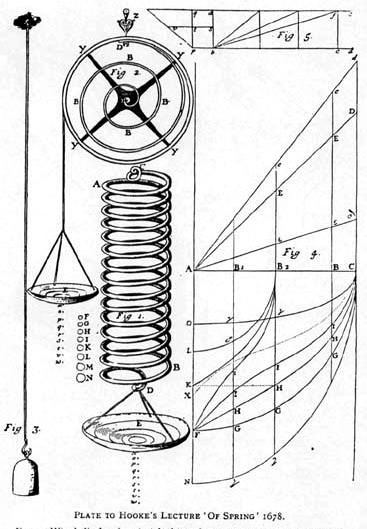
\includegraphics[height=13cm]{HookeSpring.png}
\caption{A figure from Hooke's original treaty. The applied force is proportional to the masses put in the plate of the scale. In this chapter we are substituting an elastic solid to the spring, and translating this figure into the language of tensors.}
\end{center}
\label{HookeSpring}
\end{figure}
 {\emph{Linear elasticity}} describes transformation of solids that are sufficiently small 
 to be reversible: if the force $F$ is decreased to zero after a traction experiment {\emph{in the linear 
 regime}}, the material comes back to its initial state. The amplitude of the linear regime depends on the material and on the 
 nature of the transformation (for example for steel $\delta L /L$ is of the order of a few thousands in the
linear regime, whereas for rubber it can be a few percents), and it has to be determined
 by experiment, just as Young's modulus. If $F$ is increased beyond the elasticity regime, the is a second regime
 in which the force can be decreased, while $\delta L$ decreases without going back to zero (there is a {\emph{remanent deformation}}).
 For even larger values of $F$ there is breakage. The scope course of this course is confined
 to linear elasticity.\\
 



{\bf{Remarks on gravity, linearity and orders of magnitude.}} 
 In the above discussion we did not specify the direction of the applied forces: we 
 just described them are traction forces, i.e. they are parallel to the axis of the cylinder, i.e.
 $\vec{F} = F \vec{n}$ at both ends of the cylinder, with $F>0$ for a traction ($F<0$ would be
a compression), but the normal vector $\vec{n}$ could be horizontal or vertical. This means we neglected 
 gravity (and we will often neglect it in the context of linear elasticity). There 
 are two reasons to neglect gravity:\\
1. We are interested in small deformations from an initial equilibrium state to a final equilibrium state,
  and the equilibrium equations in the initial state include gravity and the forces that balance it (for example the reaction
 of a table if the cylinder rests horizontally on a table, or the reaction of the ceiling
 if the cylinder is attached to the ceiling). So we begin our work when gravity has already been taken into account, and
 we look for variations of the stress tensor with respect to this state.\\
2. For many solids of interest, the value of Young's modulus makes gravity forces 
 smaller than traction forces by orders of magnitude, even for small deformations. In the case of steel, $E\simeq 200 \GPa$, and the traction regime is linear for $0\leq \delta L / L \leq 0.5 \times 10^{-3}$, so if we consider a cylinder of steel
 with mass $m=1 \kg$ and $S=10 \cm^2$, the effect of gravity by unit of surface 
 is about 
\[
\frac{mg}{S} = \frac{1\times 10}{10^{-3}} = 10^4 \Pa,
\]
and that of the traction force per unit surface for $\delta L / L \leq 0.5 \times 10^{-3}$ is about:
\[
\frac{F}{S} = E \frac{\delta L}{L} = 2\times 10^{11} \times 5 \times 10^{-4} = 10^8 \Pa,
\]
or $10^4$ times larger.

\section{Linearized strain tensor}
In Lecture 2 we described the kinematics of continuous media in terms of a flow $\vec{\Phi}$ that maps the initial coordinates $X_i\vec{e_i}$
of material points in a continuous medium to a new position at time $t$, with coordinates $\Phi_i( \vec{X}, t ) \vec{e_i}$.  
In the linear regime where Hooke's law (Eq. \ref{Young}) holds, deformations are small in scale of the original dimensions of the material,
 so  we will express them in terms of the displacement fields $u_i$ defined in terms of the flow
 by subtracting the identical flow:
\begin{equation}
u_i( \vec{X},t) = \Phi_i( \vec{X},t) - X_i,
\end{equation}  
so that vector fields (see the chapter on kinematics are transformed as follows 
 by the flow:
\begin{equation}
\vec{h} \mapsto \left(  T_{ij}h_j\right) \vec{e_i},
\end{equation}
with 
\begin{equation}
  T_{ij} = \frac{\partial \Phi_i}{\partial X_j} = \delta_{ij} + \frac{\partial u_i}{\partial X_j}.
\end{equation}
 We are going to assume that the components $u_i$ for all $i$ are small, and slowly varying over space (i.e. all their derivatives
 are assumed to be small).
Let us expand the deformed dot-product of vectors $h$ and $h'$ in powers of $u$:
\[
\boxed{
\begin{array}{lll}\vec{h}.\vec{h'} \mapsto& \left( T_{ij} h_j \vec{e_i} \right) .\left( T_{lk}h'_k \vec{e_l}\right) &  = h_j h'_k T_{ij} T_{lk}  \delta_{il}\\
   add my equation & = h & into this list\\
    &  &   = h_j h'_k   \left(  \delta_{ij} + \frac{\partial u_i}{\partial X_j} \right)  \left( \delta_{ik} + \frac{\partial u_i}{\partial X_k}  \right) \\
    &  & =h_j h'_k   \left(  \delta_{ij} + \frac{\partial u_i}{\partial X_j} \right)  \left( \delta_{ik} + \frac{\partial u_i}{\partial X_k}  \right)\\
    &  & = h_j h'_k   \left(  \delta_{ij} \delta_{ik} +  \delta_{ij}\frac{\partial u_i}{\partial X_k} +\frac{\partial u_i}{\partial X_j} \delta_{ik}+
 \frac{\partial u_i}{\partial X_j} \frac{\partial u_i}{\partial X_k} \right)\\
    &  & = h_j h'_k   \left(  \delta_{jk} +  \frac{\partial u_j}{\partial X_k} + \frac{\partial u_k}{\partial X_j}  + \frac{\partial u_i}{\partial X_j} \frac{\partial u_i}{\partial X_k} \right).
  \end{array}}
\label{dotTransform}
\]

 Hence we can express the first-order terms in $\vec{u}$ (and its derivatives) in terms
  of the deformation tensor $\epsilon$ defined as:
\begin{equation}
\boxed{\epsilon_{ij} (\vec{X},t)= \frac{1}{2}\left(  \frac{\partial u_i}{\partial X_j} + \frac{\partial u_j}{\partial X_i} \right)},
\label{epsilonDef}
\end{equation}
and we find:
\begin{equation}
\boxed{
\vec{h}.\vec{h'} \mapsto  \vec{h}.\vec{h'} + 2\epsilon_{ij} h_i h'_j + o (\vec{u}).
}
\end{equation}

{\bf{Example: traction of a cylinder.}} In the special case of the traction on a cylinder, the variation of length $\delta L$  is proportional 
 to the length, so for a cylinder of initial length $\alpha L$, with the same base  surface $S$ and 
 the same traction $F$, the length would vary by $\alpha \delta L$. One can express
  this proportionality rule by writing the displacement  field in the direction $\vec{e_3}$ as:
\[
u_3 = \frac{X_3}{L} \delta L,
\]
where the factor $X_3/L$ plays the role of the factor $\alpha$.
 Hence we can express one component
 of the linearized strain tensor:
\[
 \epsilon_{33} = \frac{\delta L}{L}.
\]
If we look at a section of the cylinder by a plane orthogonal to its 
 axis, we have a disk whose radius is $a=\sqrt{S/\pi}$ when $F=0$.
 This radius will be $a + \delta a $ when the traction $F$  is applied, 
with $\delta a < 0 $, and by the same reasoning as for the direction 
 $X_3$ one can convince oneself that the displacement 
 is linear in both $X_1$ and $X_2$ directions:
 \[
u_1 = \frac{X_1}{a}  \delta a,
\]
 \[
u_2 = \frac{X_2}{a}  \delta a,
\]
so that in particular,
\[
\epsilon_{11} = \epsilon_{22} = \frac{\delta a}{a}.
\]
Instead of describing this situation in terms of the radius $a$, which depends on the  
 geometry, one chooses to describe it in terms of the ratio between components of the strain tensor.
 In terms of Poisson's ratio (the parameter $\nu$ defined in Eq. \ref{PoissonDef}), for the cylinder in traction,
 and small deformations, we find:
\[
 \epsilon_{11} = \epsilon_{22} = -\nu \epsilon_{33}.
 \label{thinning}
\]
 Poisson's ratio depends on the material, and has no physical dimension. One can compute its value for an incompressible
 material (exercise, see tutorial), and measure it in traction expreriments as it equals the relative variation of the 
 radius (for example $\nu \simeq 0.28$ for steel, and $\nu = 0.2$ for concrete).



\section{Deformations as a function of stress}
%\subsection{Translation of Hooke's law into the language of tensors}

 For traction forces acting on the ends of  a cylinder,
without volume forces, the following uniaxial stress tensor is statically admissible (see Tutorial 4):
\[
\sigma(\vec{x})=  \left(
   \begin{array}{l l l}
      0  & 0   & 0 \\
      0 & 0  & 0\\
      0 & 0 & \frac{F}{S}
   \end{array}
   \right)
\label{uniaxial}
\]
Hooke's law can therefore be rewritten as the following relation between the entry $\epsilon_{33}$
 of the tensor $\epsilon$ and the entry with the same indices of the stress tensor:
\begin{equation}
\epsilon_{33} = \frac{1}{E} \sigma_{33}.
\label{HookeComponents}
\end{equation}
But this is not a relation between $\epsilon$ and $\sigma$ as matrices. We can 
 proceed by trial-and-error and ask: {\emph{"What if the relation \ref{HookeComponents} 
 held between all the entries of $\epsilon$ and $\sigma$?"}}
We would have  
\begin{equation}
\epsilon_{ij} {\whatIf^?}  \frac{1}{E} \sigma_{ij},
\label{HookeWhatIf}
\end{equation}
 which is the simplest generalization of Eq. \ref{HookeComponents} to the tensors  $\epsilon$
 and $\sigma$. But in that case, the components $\epsilon_{11}$ and $\epsilon_{22}$ of
 the deformation tensor would be zero (because $\sigma$ is uniaxial, Eq. \ref{uniaxial}), therefore the cylinder would not become thinner
 under traction, which would be in contradiction with our prediction \ref{thinning}, as we know Poisson's ratio is measured to be different 
 from zero.\\

 To account for the transverse thinning of the cylinder under traction, we therefore
 need to add other terms to the r.h.s of \ref{HookeComponents}. Linearity 
  and isotropy impose that these terms should have the same eigenvectors
 as $\sigma$ (for any choice of $\sigma$), and should be a linear function of $\sigma$. A natural 
 way to satisfy these two conditions is to add a tensor proportional 
  to the identity matrix, with the trace of $\sigma$ as a coefficient. 
 We now have two parameters, call them $E_1$ and $E_2$:
\begin{equation}
\epsilon_{ij} {\whatIf^?} \frac{1}{E_1} \sigma_{ij} + \frac{1}{E_2} (\Tr \sigma)\delta_{ij}.
\label{HookeWhatIf2}
\end{equation}
 Again we ask:  {\emph{"What if  $\epsilon$ was given by Eq. \ref{HookeWhatIf2}?"}}\\
For the cylinder in pure traction, the l.h.s. of \ref{HookeWhatIf2} equals $F/(ES)$ by Hooke's law and the 
 r.h.s. equals $F/(E_1S) + F/(E_2S)$ from the expression of the uniaxial tensor (Eq. \ref{uniaxial}).
In order to recover Hooke's law (Eq. \ref{HookeComponents}) for the cylinder in 
pure traction, we must have
 \begin{equation}
\frac{1}{E} = \frac{1}{E_1} + \frac{1}{E_2}.
\label{EE1E2}
\end{equation}
 Again for the cylinder in pure traction, we can express the diagonal terms of the deformation tensor from Eq. \ref{HookeWhatIf2} as $\epsilon_{11} = F/(E_2S)$ and $\epsilon_{22} = F/(E_2S) $,  but from our experimental definition of Poisson's ratio, they must equal $-\nu\epsilon_{33} = -\nu F/(ES)$. Hence the relation
\begin{equation}
-\frac{\nu}{E} = \frac{1}{E_2}. 
\label{nuE1E2}
 \end{equation}
By plugging Eq. \ref{nuE1E2} into Eq. \ref{EE1E2}, we can express the parameters $E_1$ and $E_2$ in terms
 of the measurable quantities $\nu$ and $E$, and conclude that the proposed form Eq. \ref{HookeWhatIf2}
 is compatible with observations in the linear regime of the traction experiment, provided the stress and strain tensors
are related by the following equation:
\begin{equation}
\boxed{\epsilon_{ij} = \frac{1+\nu}{E} \sigma_{ij} - \frac{\nu}{E} \left( \Tr\sigma \right) \delta_{ij}}.
\label{HookeTensor}
\end{equation}
 We will assume from now on that this educated guess gives us
 the relation between strain and stress in the linear regime of deformation, 
for all elastic solids, and not only in the case of pure traction but also for more general systems of applied 
 forces (see tutorials for tests of this idea in the cases of shear deformation and isotropic pressure).

\section{Stress as a function of deformation}
So far we have expressed the deformation tensor $\epsilon$ as a function of the stress 
tensor $\sigma$. In order to link dynamics to kinematics we can invert the tensor form of Hooke's law (Eq. \ref{HookeTensor}),
 and obtain the expression of the stress tensor as a function of the deformation tensor.\\

As Hooke's law can be rewritten as
\begin{equation}
 \sigma_{ij}= \frac{E}{1+\nu}\epsilon_{ij} +\frac{\nu}{1 + \nu} \left( \Tr\sigma \right) \delta_{ij},
\end{equation}
all we need to do is to express $\left( \Tr\sigma \right)$ as a function of $\epsilon$
 Let us take the trace of Eq. \ref{HookeTensor}:
\begin{equation}
 \Tr \epsilon =  \frac{1+\nu}{E} \Tr \sigma - \frac{\nu}{E}\left( \Tr\sigma \right) \delta_{ii}.
\end{equation}
As $\delta_{ii} =3$, we obtain: 
\begin{equation}
\Tr \epsilon =  \frac{1-2\nu}{E} \Tr \sigma,
\end{equation}
hence we obtain the following expression for the stress tensor:
\begin{equation}
 \boxed{\sigma_{ij}= \frac{E}{1+\nu}\epsilon_{ij} +\frac{E\nu}{(1 + \nu)(1-2\nu)} \Tr \epsilon \delta_{ij}.}
\end{equation}

\end{document}

In this lecture we will develop the mathematical description of deformations.
We will describe movements without studying its causes. This is the kinematics of 
 continuous media. A function of position and time is
 used to describe the motion of the continuous medium. 
 To decide whether the medium is deformed, we have to compute how
 scalar products of vectors change under the flow (see Fig. \ref{figur} for
 a physical example: we are going to describe how the grid on the figure is deformed).


\section{Lagrangian description of flows}
\subsection{Definitions and notations}
To avoid boundary effects, let us study a sample of continuous 
medium (solid or fluid) that "fills the entire space" (meaning we are describing
matter at scales that are large compared to the size of molecules, but we are far away from 
 the boundaries of the sample).\\

The space ${\mathbf{R}}^3$ is endowed with 
 an orthonormal base $(\vec{e_1}, \vec{e_2}, \vec{e_3})$ and a
 fixed origin, so the position of a material point $M$ can be described 
 by its coordinates, $\overrightarrow{OM} =\vec{x}= x_i\vec{e_i}$.
We are interested in the way  classical particles (small lumps of continuous medium, which could be 
visualized using tracers in a fluid, or simply by marking the surface by a grid on a solid, as in Fig. \ref{figur}) move over time. Let us say that a particle
 is at position $\vec{X}$ at time $t =0$. Its position at time $t >0$
 can be described by a vector which depends on $t$ and on the point from which the particle came.
 Let us denote this vector by $\Phi_1(\vec{X}, t) \vec{e_1} + \Phi_2( \vec{X},t)\vec{e_2} + \Phi_3( \vec{X}, t )\vec{e_3}$.
 Since we can consider any initial position $\vec{X}$, we have just defined an application $\vec{\Phi}$
 that described the movements of the continuous medium over a time between $t=0$ and $t=T$:

\begin{equation}
 {\mathbf{R}^3}\times [ 0, T] \longrightarrow {\mathbf{R}^3}
\end{equation}
\begin{equation}
 (\vec{X},t)\mapsto \vec{\Phi}( \overrightarrow{X},t) = \Phi_1(\vec{X}, t) \vec{e_1} + \Phi_2( \vec{X},t) \vec{e_2} + \Phi_3( \vec{X}, t ) \vec{e_3}.
\label{flowDef}
\end{equation}

\begin{figure}[htp]
 \centering

  \begin{tabular}{cc}

    % Requires \usepackage{graphicx}

    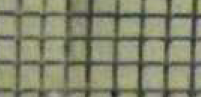
\includegraphics[width=60mm]{recGrid.png}&

    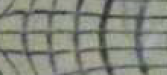
\includegraphics[width=60mm]{recGridPrime.png}\\
  \end{tabular}
\label{figur}\caption{A sample of perspex with 
 orthogonal lines drawn with a pen at $t=0$, and and $t>0$ after traction.}

\end{figure}

\subsection{Computing the tangent to a curve in three dimensions} 
Let us start at a point $\vec{X}$ in the continuous medium, at time $t=0$.
 We can move around this vector by adding a vector $\vec{h}$ to it.
 We will need  to do differential calculus (in order to compute tangent vectors), so let us introduce a scalar parameter
 $s\in \mathbf{R}$, which we will eventually let go to 0.\\
The vector $\vec{h}$ is the tangent vector of the straight line that
 goes through $X$ in direction $\vec{h}$, as we have
\begin{equation}
 \frac{1}{s}\left( (\vec{X}+ s\vec{h} ) - \vec{X}\right)\longrightarrow_{s\rightarrow 0} \vec{h}.
 \label{tangentFirst}
\end{equation}
 What does this situation look like at time $t>0$?\\
By definition of the flow, the  particle that was at $\vec{X}$ 
 is now at $\vec{\Phi}(t)$ and the particle that was at $\vec{X}+ s\vec{h}$ 
 is now at $\vec{\Phi}(\vec{X}+ s\vec{h},t)$, 
 so the quantity we studied in Eq. \ref{tangentFirst}
 has now become
\begin{equation}
 \frac{1}{s}\left( \vec{\Phi}(\vec{X}+ s\vec{h},t) -  \vec{\Phi}(\vec{X},t) \right)
 \label{accrFinal}
\end{equation}
 Let us study its limit when $s$ goes to zero, which is\footnote{As an exercise, the 
 reader should put the symbols $\vec{X}, \vec{h}, \vec{\Phi}(\vec{X},t),\vec{\Phi}(\vec{X}+\vec{h},t)$ on Fig. \ref{figur}, and draw the two curves we 
 are talking about.}  the tangent 
 to the curve $s \in \mathbf{R} \mapsto   \vec{\Phi}(\vec{X}+ s\vec{h},t)$.\\
 

Let us write all the components in matrix form in the base $\eBase$
to compute this tangent:
\begin{equation}
\vec{\Phi}(\vec{X}+ s\vec{h},t) -  \vec{\Phi}(\vec{X},t) =   \left(
   \begin{array}{l}
       \Phi_1(\vec{X}+ s\vec{h},t) - \Phi_1(\vec{X},t)\\
      \Phi_2(\vec{X}+ s\vec{h},t) - \Phi_2(\vec{X},t)  \\
       \Phi_3(\vec{X}+ s\vec{h},t) - \Phi_3(\vec{X},t)\\
   \end{array}
   \right)
\label{accrVector}
\end{equation}

Let us assume that the components of $\vec{\Phi}$ are smooth functions (they posess
derivatives at all orders). One can write a first-order Taylor expansion 
 of each of the  components of the vector in Eq. \ref{accrVector}. For example:
\begin{equation}
 \Phi_1(\vec{X}+ s\vec{h},t)  = \Phi_1(\vec{X},t) + s h_1 \frac{\partial\Phi_1}{\partial X_1}(\vec{X},t) + s h_2 \frac{\partial\Phi_1}{\partial X_2}(\vec{X},t)+
   s h_3 \frac{\partial\Phi_1}{\partial X_3}(\vec{X},t) + o(s).
\end{equation}
Hence the quantity 
\begin{equation}
 \frac{1}{s}\left(\Phi_1(\vec{X}+ s\vec{h},t)  - \Phi_1(\vec{X},t) \right) =  h_1 \frac{\partial\Phi_1}{\partial X_1}(\vec{X},t) +  h_2 \frac{\partial\Phi_1}{\partial X_2}(\vec{X},t)+
   h_3 \frac{\partial\Phi_1}{\partial X_3}(\vec{X},t) + \frac{o(s)}{s},
\end{equation}
 and its limit when $s$ goes to zero is given by:
\begin{equation}
h_i \frac{\partial \Phi_1( \vec{X})}{\partial X_i}.
\end{equation}
 The computation can be repeated for $\Phi_2$ and $\Phi_3$, and one obtains the following limit:
\begin{equation}
\frac{1}{s}\left(
\vec{\Phi}(\vec{X}+ s\vec{h},t) -  \vec{\Phi}(\vec{X},t)\right) \longrightarrow_{s\rightarrow 0}   \left(
   \begin{array}{l}
      h_i \frac{\partial \Phi_1( \vec{X})}{\partial X_i}\\
     h_i \frac{\partial \Phi_2( \vec{X})}{\partial X_i}\\
     h_i \frac{\partial \Phi_3( \vec{X})}{\partial X_i}
   \end{array}
 \right).
\end{equation}
%\boxed{
 Hence the vector $\vec{h} = h_j\vec{e_j}$ is mapped to 
 the vector 
\begin{equation}
h_i \frac{\partial \Phi_j( \vec{X})}{\partial X_i} \vec{e_j} = h_i T_{ji} \vec{e_j}.
\label{transportVec}
\end{equation}
 by the flow, where we have defined 
 the matrix $T$ by:\\
\begin{equation}
 T_{ij} =  \frac{\partial \Phi_i( \vec{X})} {\partial X_j},
 \label{equation}
\end{equation}
which maps vectors from position $\vec{X}$ to position $\vec{\Phi}(\vec{X},t)$.
 $T$ is called the {\emph{strain tensor}}.
%}

\section{How does the scalar product change under the flow?}

 Taking a pair of vectors $\vec{h} = h_i\vec{e_i}$ and $\vec{h'} = h'_i \vec{e_i}$
 starting from position $\vec{X}$, one can transport both vectors by the flow
 using Eq. \ref{transportVec}, and compute the dot-product of the resulting vectors:\\
\begin{equation}
 \left( h_i \frac{\partial \Phi_j( \vec{X})}{\partial X_i} \vec{e_j} \right) .\left( h_k \frac{\partial \Phi_l( \vec{X})}{\partial X_k} \vec{e_l}\right) = h_i h_k\frac{\partial \Phi_j( \vec{X})}{\partial X_i}\frac{\partial \Phi_l( \vec{X})}{\partial X_k}\delta_{jl} =  h_i h_k\frac{\partial \Phi_j( \vec{X})} {\partial X_i}\frac{\partial \Phi_j( \vec{X})}{\partial X_k}.
\label{dotTransform}
\end{equation}


 One could be tempted to say that there is "no deformation" if the matrix $T$ is the identity matrix. However this
condition is too restrictive. Indeed we can see from Eq. \ref{dotTransform}
 that if $T_{ji}T_{jk} = \delta_{ik}$, the scalar product is preserved (hence the grid drawn on Fig. \ref{figur}
 is not deformed, just rotated).    Hence we see that the local deformations
 are measured by the measured by the difference $T_{ji}T_{jk} - \delta_{ik}$.







\end{document}

 A new state of equilibrium at $t>0$



to-do: 
- biographical notices
- uniaxial
